
    \begin{picture} (300.000000,132.375000)(0,0)
    \put(0.0, 0.0){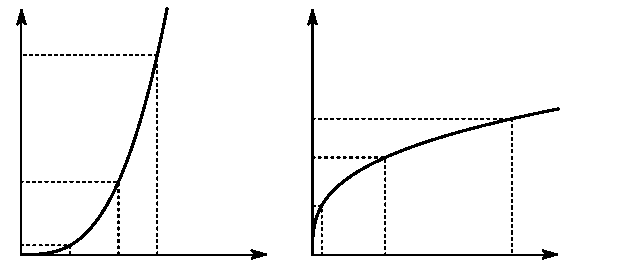
\includegraphics{01inversefunctions.pdf}}
        \put( 33.59,   0.31){\sffamily\itshape \makebox[0pt][c]{$a$}}
    \put(  8.31,  14.68){\sffamily\itshape \makebox[0pt][r]{$f(a)$}}
    \put(154.37,   0.31){\sffamily\itshape \makebox[0pt][c]{$f(a)$}}
    \put(148.00,  33.59){\sffamily\itshape \makebox[0pt][r]{$a$}}
    \put( 56.88,   0.31){\sffamily\itshape \makebox[0pt][c]{$b$}}
    \put(  8.31,  45.23){\sffamily\itshape \makebox[0pt][r]{$f(b)$}}
    \put(184.92,   0.31){\sffamily\itshape \makebox[0pt][c]{$f(b)$}}
    \put(148.00,  56.88){\sffamily\itshape \makebox[0pt][r]{$b$}}
    \put( 75.50,   0.31){\sffamily\itshape \makebox[0pt][c]{$c$}}
    \put(  8.31, 106.14){\sffamily\itshape \makebox[0pt][r]{$f(c)$}}
    \put(245.83,   0.31){\sffamily\itshape \makebox[0pt][c]{$f(c)$}}
    \put(148.00,  75.50){\sffamily\itshape \makebox[0pt][r]{$c$}}
    \put( 14.97, 131.38){\sffamily\itshape The graph of $f$}
    \put(163.97,  94.12){\sffamily\itshape The graph of $f^{-1}$}
\end{picture}
